\section{FSM}
Beim Modellieren von Zustandsmaschinen kommen grundsätzlich Zustandsdiagram oder Statecharts in frage. 
Dabei sind \textbf{Zustandsdiagramme} einfacher, können aber keine Hierarchieen, nebenläufige Prozesse oder Braodcastkommunikationen abbilden.
\begin{center}
	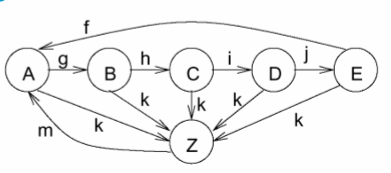
\includegraphics[width=0.8\columnwidth]{Images/zustandsdiagramm}
\end{center}


Bei Statecharts können Historie mechanism verwendet werden, wobei beim erneuten eintreten in ein Sub-State, den Initial State oder den letzten State ausgeführt werden. Beim Deep-History, merkt sich der Zustand bis in die unterste Ebene, in welchem er war, bei Shallow werden die unteren mit dem Initial Zustand ausgewührt.
\begin{center}
	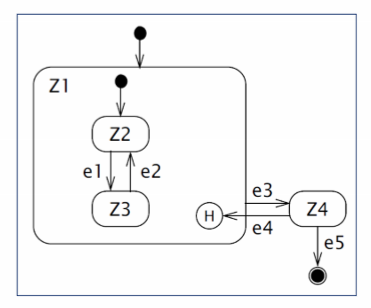
\includegraphics[width=0.8\columnwidth]{Images/statechart}
\end{center}

\begin{center}
	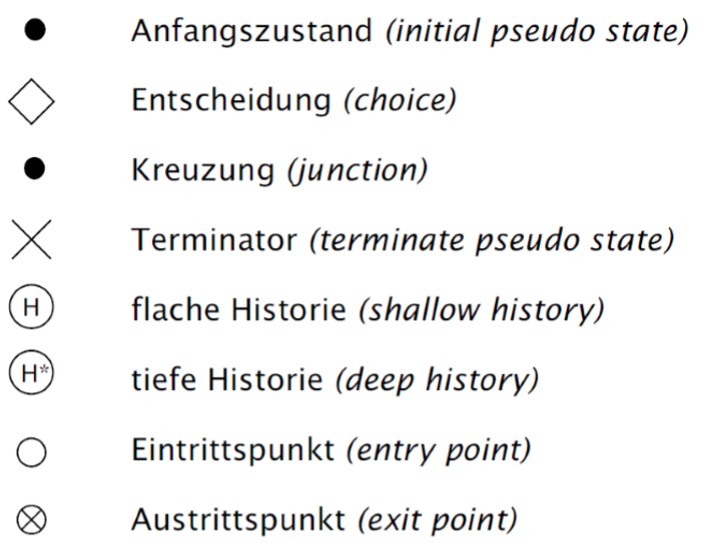
\includegraphics[width=0.8\columnwidth]{Images/statechart_elemente}
\end{center}

\subsection{Realisierung}
Eine FSM wird häufig durch switch-Case, Tabellen, State-Pattern oder generischen Templates umgesetzt. Siehe Anhang.